\subsection{Geração de biomas no diagrama de Voronoi}
\label{sec:geracao_procedural_biomas}

Biomas são regiões ecológicas que possuem fauna e flora com atributos estruturais semelhantes \cite{maestrovirtuale}. Segundo \citeonline{amitp2010}, gera-se um mapa e seus biomas definindo-se o litoral, sendo este a borda que separa a água do solo. Na \cref{fig:voronoi-land-water}, mostra-se essa separação, sendo os polígonos marrons representando o solo e os polígonos azuis representando o mar.

É possível utilizar qualquer formato para gerar as ilhas, como formas geométricas e funções de ruídos como o Perlin Noise \cite{amitp2010}.

\begin{figure}[ht]
	\caption{Diagrama de Voronoi separado em solo e mar}
	\centering % para centralizarmos a figura
	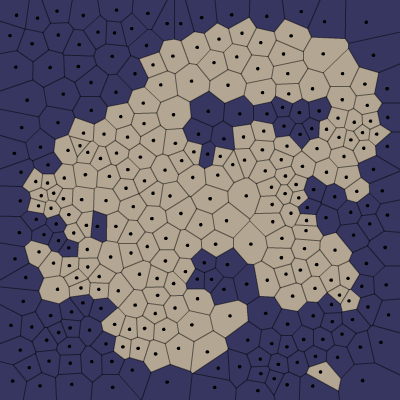
\includegraphics[width=0.8\textwidth]{figures/voronoi-land-water.png} % leia abaixo
	\legend{Fonte: \citeonline{amitp2010}}
	\label{fig:voronoi-land-water}
\end{figure}

A elevação do mapa é definida pelos cantos dos polígonos e é calculada através da distância de todos os polígonos indicados como solo até o litoral \cite{amitp2010}. A \cref{fig:downslopes} representa essa elevação, sendo os polígonos azuis o mar, os níveis da elevação são os polígonos de verde (mais baixo) a branco (mais alto), e as setas indicam as direções das encostas.

\begin{figure}[ht]
	\caption{Diagrama de Voronoi separado em solo e mar com os cantos dos polígonos indicando a direção para o litoral}
	\centering
	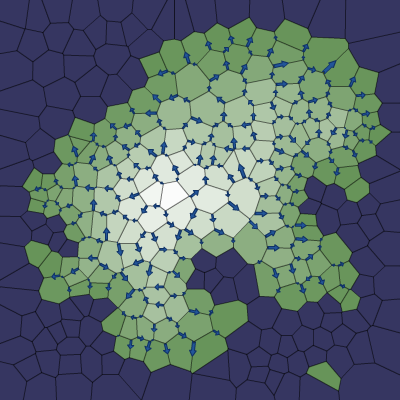
\includegraphics[width=0.7\textwidth]{figures/downslopes.png}
	\legend{Fonte: \citeonline{amitp2010}}
	\label{fig:downslopes}
\end{figure}

A elevação é utilizada para gerar os biomas. Por exemplo, elevações altas indicam montanhas, que, consequentemente, devem possuir neve. Adicionando mais uma camada, além da elevação, como a de umidade, podemos gerar uma variedade maior de biomas. A umidade é calculada com base na distância do polígono a um corpo d'água \cite{amitp2010}.

\subsection*{Diagrama de Whittaker}

O diagrama de Whittaker é uma forma de dividir os terrenos gerados a partir da técnica de geração procedural. Esse diagrama inclui valores de temperatura e umidade para separar os biomas, conforme exemplificado na \cref{fig:diagrama-whittaker} \cite{wikidotwhittakerdiagram}.

\begin{figure}[ht]
	\caption{Diagrama de Whittaker}
	\centering
	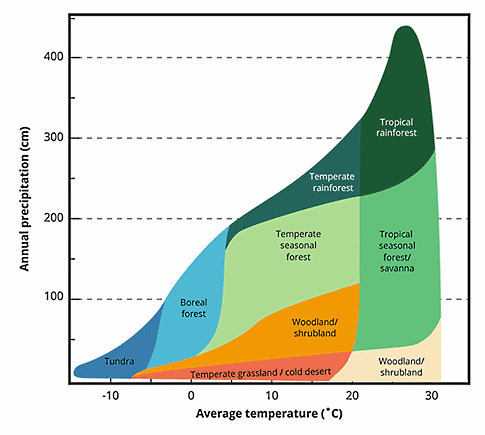
\includegraphics[width=0.6\textwidth]{figures/diagrama-whittaker.png}
	\legend{Fonte: \citeonline{mendes2019}}
	\label{fig:diagrama-whittaker}
\end{figure}

Utilizando a elevação como representante da temperatura de um bioma, é possível empregar o diagrama de Whittaker. Fazendo ajustes nesse diagrama, é possível adicionar ou remover biomas. Com essa nova camada, torna-se possível a adição de rios ao mapa \cite{amitp2010}, resultando no mapa final apresentado na \cref{fig:biomes}.

\begin{figure}[ht]
	\caption{Resultado final da geração do mapa}
	\centering
	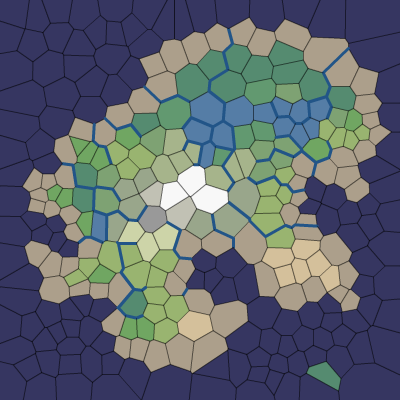
\includegraphics[width=0.5\textwidth]{figures/biomes.png}
	\legend{Fonte: \citeonline{amitp2010}}
	\label{fig:biomes}
\end{figure}
